\chapter{Rekurzia}
\label{sec:rekurzia}
\def\stringcolor{solarized@blue}
\def\longSierp{1}

Volanie funkcie pri vyhodnocovaní výrazu, ako sme ho opísali v minulej kapitole,
nemusí byť len z hlavného programu, ale z hocijakej funkcie, tento program
vypíše 16:\\

\vbox{
\begin{lstlisting}[] 
#include <iostream>
using namespace std;

int a(int x) { return x + 1; }

int b(int x) { return a(x) * a(x); }

int main() { cout << b(3) << endl; }
\end{lstlisting}
}

Jediná vec, ktorú treba dodržať je, podobne ako pri premenných, že každé použitie
(volanie) musí byť až vtedy, keď funkcia bola v programe vyrobená. Keby si
napr. v predchádzajúcom programe prehodil riadky s definíciou funkcií \vb{a} a \vb{b},
nefungoval by. 

 Špeciálne zaujímavá je situácia, keď funkcia vo svojom tele volá sama seba. Takéto
volanie je možné a hovorí sa mu {\em rekurzia}. Na prvý pohľad to možno vyzerá divne, ale
nie je to. Treba len, podobne ako pri cykle, zabezpečiť, aby sa volanie nezacyklilo
ako táto funkcia:\\

\vbox{
\begin{lstlisting}[] 
int a(int x) { return 1 + a(x + 1); }
\end{lstlisting}
}

Čo sa začne diať, ak zavoláš \prg!a(0)!? Najprv sa spraví nový svet funkcie \prg!a!,
v ktorom sa \vb{x} nastaví na 0 a začne sa vykonávať telo funkcie. V ňom
sa spraví nový nezávislý svet funkcie \vb{a}, v ktorom sa  \vb{x} nastaví na 1
a začne sa vykonávať telo funkcie. V ňom
sa spraví nový nezávislý svet funkcie \vb{a}, v ktorom sa  \vb{x} nastaví na 2
a začne sa vykonávať telo funkcie. V ňom
sa spraví nový nezávislý svet funkcie \vb{a}, v ktorom sa \ldots



Keď ale funkcii naprogramuješ správne ''dno'', niektoré rekurzívne zápisy
sú veľmi prirodzené. Zober si napríklad hľadanie najväčšieho spoločného deliteľa.\indexItem{Mat}{najväčší spoločný deliteľ}%
Euklides vedel, že ak máme dve čísla $a$ a $b$ také, že $a>b$, 
a obidve sú deliteľné číslom $k$,
to znamená že $a=xk$ a $b=yk$ pre nejaké $x$ a $y$. Potom $a-b=xk-yk=(x-y)k$,
a teda aj $x-y$ je deliteľné číslom $k$. Preto každý spoločný deliteľ $a$ a $b$
je zároveň spoločným deliteľom $a-b$ a $b$. Najväčšieho spoločného deliteľa
preto vieme nájsť takto:\\

\vbox{
\begin{lstlisting}[] 
int NSD(int a, int b) {
  if (a == b) return a;
  if (a == 1 || b == 1) return 1;
  if (a > b) return NSD(a - b, b);
  return NSD(b - a, a);
}
\end{lstlisting}
}

Keď zavoláme napr \prg!NSD(4,6)!, toto volanie následne zavolá \prg!NSD(2,4)!,
toto zase \prg!NSD(2,2)! a toto volanie už ďalší svet \vb{NSD} nevytvorí,
ale vráti 2. Potom už reťazovo všetky ostatné volania dobehnú a vrátia 2.
Ako sa presvedčíme, že sa táto funkcia nikdy nezacyklí? Všimni si, že keď
funkciu zavoláme s hocijakými $a>0$, $b>0$, každé ďalšie volanie zmenší
súčet $a+b$. Zároveň ani $a$, ani $b$ neklesne na nulu (to by museli byť 
v predchádzajúcom volaní rovnaké, ale vtedy by sa už ďalšie volanie nevyrobilo).
Keďže súčet nemôže klesať donekonečna, vidíme, že funkcia sa nikdy nezacyklí.

\begin{uloha}
  Napíš program, ktorý načíta zo vstupu jedno prirodzené číslo a vypíše ho otočené\footnote{%
To znamená, že najprv sa vypíše posledná cifra, t.j. zvyšok po delení desiatimi a potom
  otočené zvyšné cifry, t.j. otočená celočíselná časť po delení desiatimi.}
  Má to ale háčik: v celom programe môžeš použiť iba jedinú premennú (tú, do 
  ktorej načítaš vstup).
\end{uloha}

 S rekurziu sa často stretneš pri definícii rôznych výrazov. Napríklad takto:
\indexItem{Alg}{parsovanie výrazov}

\begin{uloha}
  \label{uloha:vyrazy}
  Zjednodušený výraz je buď jednociferné číslo, alebo má tvar 
  \vb{($\clubsuit$+$\heartsuit$)},
  alebo
  \vb{($\clubsuit$*$\heartsuit$)},
  kde \vb{$\clubsuit$} a \vb{$\heartsuit$} sú zjednodušené
  výrazy. Na vstupe zjednodušený výraz končí znakom \vb{\$}. 
  Napíš program, ktorý prečíta zo vstupu zjednodušený výraz a vyráta jeho
  hodnotu.
\end{uloha}

Zo zadania vidíme, že zjednodušené výrazy sú napr. \vb{4\$} alebo
alebo \vb{(2+((3*2)+(1+(6*3))))\$}, ale nie \vb{12\$} (nie je jednociferné), ani 
\vb{5+1\$} (nie je v zátvorkách), ani \vb{(3+8+1)\$}. 
Na čítanie vstupu použijeme premennú typu \prg!char c;! (pozri kapitolu \ref{sect:cisla}).
Príkaz \prg!cin >> c;! prečíta jeden znak zo vstupu\footnote{%
Ako sme v kapitole \ref{sect:cisla} hovorili, pri načítavaní sa preskakujú whitespace
znaky.\indexItem{Prg}{\vb{noskipws}}Toto správanie sa dá prepnúť,
ak z \prg!cin! načítaš špeciálnu hodnotu \prg!noskipws!, t.j. \prg!cin >> noskipws;!
spôsobí, že sa budú načítavať všetky znaky vrátane medzier.
}. Ak je tento znak číslica, t.j.
\prg!c>='0' && c<='9'!, tak hodnota výrazu je číslo, ktoré táto číslica reprezentuje,
t.j. \prg!c-'0';! (tu využívame, že v ASCII tabuľke idú znaky číslic za sebou).
Ak prvý znak nebola číslica, musela to byť otváracia zátvorka. Hodnotu výrazu potom
získame tak, že rekurzívne vyhodnotíme prvý výraz, prečítame znak operácie, rekurzívne
vyhodnotíme druhý výraz a vrátime výsledok (predtým ale nezabudneme prečítať
zatváraciu zátvorku). Výsledok by mohol vyzerať takto:

%\vbox{
\begin{lstlisting}[] 
int vyraz() {
  char c;
  cin >> c;
  if (c >= '0' && c <= '9') return c - '0';
  int v1 = vyraz(); // rekurzívne volanie 
  cin >> c;         // operátor
  int v2 = vyraz(); // druhé rekurzívne volanie 
  int vysledok;
  if (c == '+') 
      vysledok = v1 + v2;
  else  
      vysledok = v1 * v2;
  cin >> c;         // zatváracia zátvorka
  return vysledok;
}
\end{lstlisting}
%}

  \def\h{1.6}
  \def\w{3.2}
  \def\vyr#1{\node at (0.5*\w,-\h-0.3) {\vb{#1}};}
  \def\gr{gray!70}
  \def\lcx{0.8}
  \def\lcy{-0.6}

Poďme sa pozrieť, čo sa stane, ak zavoláš \vb{vyraz()} a na vstupe bude \vb{(2+(3*5))}. Najprv sa vytvorí svet pre funkciu \vb{vyraz()}, v ňom sa načíta znak \prg!'('!
do premennej
\vb{c}, zistí sa, že to nie je číslica, tak sa príde na príkaz \prg!int v1 = vyraz();!. Tu sa spracovanie preruší a vyrobí sa nový svet (nezávislej inštancie) funkcie 
\vb{vyraz()}. Ten má svoju vlastnú premennú \vb{c}, do ktorej sa načíta znak \prg!'2'! zo vstupu. Keďže je to číslica, vráti sa hodnota \vb{2} a svet zanikne.
Teraz sa výpočet vrátil do prvého sveta, ktorý pokračuje tam, kde prestal. Do premennej \vb{c} sa načíta ďalší znak zo vstupu, teraz je to \prg!'+'!
a príde sa na príkaz \prg!int v2 = vyraz();!.\\ 


\begin{tikzpicture}\fsc
  \def\clr{teal}
  \vyr{\textcolor{\clr}{(}2+(3*5))}
  \fr{vyraz}
  \var(4ex,-2ex){c}{\vb{\textcolor{\stringcolor}{\small '('}}}{vC}  
  \node [anchor=south west] at (0,-10ex) {\vb{v1 = vyraz();} };
  \draw[draw=\clr](0,-\h) -- (\w,-\h); 

  \begin{scope}[shift={(5.5,0)}]
    \def\clr{teal}
    \fr{vyraz}
    \var(4ex,-2ex){c}{\vb{\textcolor{\stringcolor}{\small '('}}}{vC}  
    \node [anchor=south west] at (0,-10ex) {\vb{v1 = vyraz();} };
    \draw[draw=\clr](0,-\h) -- (\w,-\h); 
    \begin{scope}[shift={(\lcx,\lcy)}]
      \def\clr{orange}
      \vyr{\textcolor{\gr}{(}\textcolor{\clr}{2}+(3*5))}
      \fr{vyraz}
      \var(4ex,-2ex){c}{\vb{\textcolor{\stringcolor}{\small '2'}}}{vC}  
      \node [anchor=south west] at (0,-10ex) {\vb{return c - '0';} };
      \draw[draw=\clr](0,-\h) -- (\w,-\h); 
    \end{scope}
  \end{scope}

  \begin{scope}[shift={(11.5,0)}]
    \def\clr{teal}
    \vyr{\textcolor{\gr}{(2}\textcolor{\clr}{+}(3*5))}
    \fr{vyraz}
    \var(4ex,-2ex){c}{\vb{\textcolor{\stringcolor}{\small '+'}}}{vC}  
    \var(14ex,-2ex){v1}{\vb{2}}{vV}  
    \node [anchor=south west] at (0,-10ex) {\vb{v2 = vyraz();} };
    \draw[draw=\clr](0,-\h) -- (\w,-\h); 
  \end{scope}

\end{tikzpicture}


Opäť sa práca preruší, vytvorí sa nezávislý svet a načíta sa 
znak. Keďže je to \prg!'('!, pokračuje sa až po volanie \prg!v1 = vyraz();!.
Opäť sa vytvorí nový svet (dva svety už čakajú prerušené) a spustí sa funkcia \vb{vyraz}. 
Prečíta sa číslica \prg!'3'! a do predchádzajúceho sveta vráti sa číslo \vb{3}. Druhý svet pokračuje, 
prečíta znak \prg!'*'! a príde na volanie \prg!int v2 = vyraz();!


\begin{tikzpicture}\fsc
    \def\clr{teal}
    \fr{vyraz}
    \var(4ex,-2ex){c}{\vb{\textcolor{\stringcolor}{\small '+'}}}{vC}  
    \var(14ex,-2ex){v1}{\vb{2}}{vV}  
    \node [anchor=south west] at (0,-10ex) {\vb{v2 = vyraz();} };
    \draw[draw=\clr](0,-\h) -- (\w,-\h); 
    \begin{scope}[shift={(\lcx,\lcy)}]
      \def\clr{magenta}
      \vyr{\textcolor{\gr}{(2+}\textcolor{\clr}{(}3*5))}
      \fr{vyraz}
      \var(4ex,-2ex){c}{\vb{\textcolor{\stringcolor}{\small '('}}}{vC}  
      \node [anchor=south west] at (0,-10ex) {\vb{v1 = vyraz();} };
      \draw[draw=\clr](0,-\h) -- (\w,-\h); 
    \end{scope}

  \begin{scope}[shift={(5.5,0)}]
    \def\clr{teal}
    \fr{vyraz}
    \var(4ex,-2ex){c}{\vb{\textcolor{\stringcolor}{\small '+'}}}{vC}  
    \node [anchor=south west] at (0,-10ex) {\vb{v2 = vyraz();} };
    \draw[draw=\clr](0,-\h) -- (\w,-\h); 
    \begin{scope}[shift={(\lcx,\lcy)}]
      \def\clr{magenta}
      \fr{vyraz}
      \var(4ex,-2ex){c}{\vb{\textcolor{\stringcolor}{\small '('}}}{vC}  
      \node [anchor=south west] at (0,-10ex) {\vb{v1 = vyraz();} };
      \draw[draw=\clr](0,-\h) -- (\w,-\h); 
      \begin{scope}[shift={(\lcx,\lcy)}]
        \def\clr{green!50!black}
        \vyr{\textcolor{\gr}{(2+(}\textcolor{\clr}{3}*5))}
        \fr{vyraz}
        \var(4ex,-2ex){c}{\vb{\textcolor{\stringcolor}{\small '3'}}}{vC}  
        \node [anchor=south west] at (0,-10ex) {\vb{return c - '0';} };
        \draw[draw=\clr](0,-\h) -- (\w,-\h); 
      \end{scope}
    \end{scope}
  \end{scope}
  
  \begin{scope}[shift={(11.5,0)}]
    \def\clr{teal}
    \fr{vyraz}
    \var(4ex,-2ex){c}{\vb{\textcolor{\stringcolor}{\small '+'}}}{vC}  
    \var(14ex,-2ex){v1}{\vb{2}}{vV}  
    \node [anchor=south west] at (0,-10ex) {\vb{v2 = vyraz();} };
    \draw[draw=\clr](0,-\h) -- (\w,-\h); 
    \begin{scope}[shift={(\lcx,\lcy)}]
      \def\clr{magenta}
      \vyr{\textcolor{\gr}{(2+(3}\textcolor{\clr}{*}5))}
      \fr{vyraz}
      \var(4ex,-2ex){c}{\vb{\textcolor{\stringcolor}{\small '*'}}}{vC}  
      \var(14ex,-2ex){v1}{\vb{3}}{vV}  
      \node [anchor=south west] at (0,-10ex) {\vb{v2 = vyraz();} };
      \draw[draw=\clr](0,-\h) -- (\w,-\h); 
    \end{scope}
  \end{scope}
\end{tikzpicture}


Teraz sa zase spraví nový svet, ktorý načíta číslo \vb{5}. Dočíta sa zátvorka a vráti sa výsledok \vb{15}.
Pôvodný svet dočíta poslednú zátvorku a vráti výsledok \vb{17}.

\begin{tikzpicture}\fsc
  \begin{scope}[shift={(0,0)}]
    \def\clr{teal}
    \fr{vyraz}
    \var(4ex,-2ex){c}{\vb{\textcolor{\stringcolor}{\small '+'}}}{vC}  
    \var(14ex,-2ex){v1}{\vb{2}}{vV}  
    \node [anchor=south west] at (0,-10ex) {\vb{v2 = vyraz();} };
    \draw[draw=\clr](0,-\h) -- (\w,-\h); 
    \begin{scope}[shift={(\lcx,\lcy)}]
      \def\clr{magenta}
      \fr{vyraz}
      \var(4ex,-2ex){c}{\vb{\textcolor{\stringcolor}{\small '*'}}}{vC}  
      \var(14ex,-2ex){v1}{\vb{3}}{vV}  
      \node [anchor=south west] at (0,-10ex) {\vb{v2 = vyraz();} };
      \draw[draw=\clr](0,-\h) -- (\w,-\h); 
      \begin{scope}[shift={(\lcx,\lcy)}]
        \def\clr{orange!50!green}
        \vyr{\textcolor{\gr}{(2+(3*}\textcolor{\clr}{5}))}
        \fr{vyraz}
        \var(4ex,-2ex){c}{\vb{\textcolor{\stringcolor}{\small '5'}}}{vC}  
        \node [anchor=south west] at (0,-10ex) {\vb{return c - '0';} };
        \draw[draw=\clr](0,-\h) -- (\w,-\h); 
      \end{scope}
    \end{scope}
  \end{scope}

  \begin{scope}[shift={(5.5,0)}]
    \def\clr{teal}
    \fr{vyraz}
    \var(4ex,-2ex){c}{\vb{\textcolor{\stringcolor}{\small '+'}}}{vC}  
    \var(14ex,-2ex){v1}{\vb{2}}{vV}  
    \node [anchor=south west] at (0,-10ex) {\vb{v2 = vyraz();} };
    \draw[draw=\clr](0,-\h) -- (\w,-\h); 
    \begin{scope}[shift={(\lcx,\lcy)}]
      \def\clr{magenta}
      \vyr{\textcolor{\gr}{(2+(3*5}\textcolor{\clr}{)})}
      \fr{vyraz}
      \var(4ex,-2ex){c}{\vb{\textcolor{\stringcolor}{\small '*'}}}{vC}  
      \var(14ex,-2ex){v1}{\vb{3}}{vV}  
      \var(14ex,-5.5ex){v2}{\vb{5}}{vV}  
      %\node [anchor=south west] at (0,-10ex) {\vb{v1 = vyraz();} };
      \draw[draw=\clr](0,-\h) -- (\w,-\h); 
    \end{scope}
  \end{scope}
    
  \begin{scope}[shift={(11.5,0)}]
    \def\clr{teal}
    \vyr{\textcolor{\gr}{(2+(3*5)}\textcolor{\clr}{)}}
    \fr{vyraz}
    \var(4ex,-2ex){c}{\vb{\textcolor{\stringcolor}{\small '+'}}}{vC}  
    \var(14ex,-2ex){v1}{\vb{2}}{vV}  
    \var(14ex,-5.5ex){v2}{\vb{15}}{vV}  
    \draw[draw=\clr](0,-\h) -- (\w,-\h); 
  \end{scope}

\end{tikzpicture}


Počas rekurzie vzniká veľa na sebe  nezávislých svetov (v našom príklade boli na sebe najviac tri, 
ale pre iné vstupy ich môže byť oveľa viac) tej istej funkcie, ktoré všetky čakajú, kým ten 
aktuálny práve ráta. Počet čakajúcich svetov sa niekedy volá {\em hĺbka rekurzie}.


Keby si chcel mať viacciferné čísla, uvedom si, že napr. hodnota čísla \prg!'4567'! je
desaťkrát hodnota čísla \prg!'456'! plus hodnota cifry \prg!'7'!.

\begin{uloha}
  Uprav predchádzajúce riešenie tak, aby pracovalo s viaccifernými číslami.
\end{uloha}


\begin{column}{0.6}
Niekedy je dobé mať globálnu premennú (napr. pole), do ktorého rekurzívna funkcia 
postupne generuje všetky možnosti: skúsi prvú možnosť, rekurzívne doplní zvyšok, skúsi
druhú možnosť, atď. Napríklad chcem pre zadané \vb{n}  vypísať všetky
$n$-bitové čísla v dvojkovej sústave, napr. v poradí ako vpravo.
Vypísať všetky čísla môžem tak, že najprv vypíšem všetky, ktoré sa začínajú nulou a potom
všetky, ktoré sa začínajú jednotkou. Všetky $n$-bitové čísla, ktoré sa začínajú nulou, viem
vypísať tak, že vypíšem všetky \vb{n-1}-bitové čísla, akurát že pred každým napíšem nulu.
Ako to naprogramovať pomocou rekurzie? 
\end{column}\hfill\begin{column}{0.3}
\begin{outputBox}
0 0 0 
0 0 1 
0 1 0 
0 1 1 
1 0 0 
1 0 1 
1 1 0 
1 1 1 
\end{outputBox}
\end{column}

Urobím si pole, v ktorom bude \vb{n} čísel. 
Začnem tak, že na prvé miesto napíšem nulu a rekurzívne sa zavolám na zvyšok. Budem ale potrebovať
písať na iné miesta v poli, preto moja funkcia bude mať ako parameter císlo miesta poľa, na ktoré
má zapisovať. Keď sa v rekurzii dostanem až na koniec poľa, jednoducho ho vypíšem. Mohlo by to 
vyzerať napr. takto:

%\vbox{
\begin{lstlisting}
#include <iostream>
using namespace std;

int a[100];
int n;

void vypis(int k) {
  if (k == n) {
    for (int i = 0; i < n; i++) cout << a[i] << " ";
    cout << endl;
  } else {
    a[k] = 0;
    vypis(k + 1);
    a[k] = 1;
    vypis(k + 1);
  }
}

int main() {
  cin >> n;
  vypis(0);
}
\end{lstlisting}
%}

\indexItem{Alg}{Grayov kód}
Čo ak teraz chcem, aby som čísla vypisoval v takom poradí, že sa vždy zmení iba jedna 
cifra\footnote{takéto usporiadanie sa volá Grayov kód}, napr:

\begin{outputBox}
0 0 0 
0 0 1 
0 1 1 
0 1 0 
1 1 0 
1 1 1 
1 0 1 
1 0 0 
\end{outputBox}

Všimni si, že ten výpis má podobnú vlastnosť, ako ten minulý: najprv idú všetky čísla, ktoré
sa začínajú nulou, a potom všetky také, ktoré sa začínajú jednotkou. Akurát, že tie jednotkové
musím vypisovať v opačnom poradí. Ako to jednoducho v rekurzii docielim? Namiesto toho, aby som 
najprv napísal nulu a potom jednotku stačí, aby som najprv nechal číslo, ktoré tam bolo pôvodne 
(predpokladám, že na začiatku mám v poli samé nuly) a potom opačné číslo. 
Premysli si, prečo je to tak.
Výsledok by teda mohol byť:

\vskip 2ex
%\vbox{
\begin{lstlisting}
#include <iostream>
using namespace std;

int a[100];
int n;

void vypis(int k) {
  if (k == n) {
    for (int i = 0; i < n; i++) cout << a[i] << " ";
    cout << endl;
  } else {
    vypis(k + 1);
    a[k] = 1 - a[k];
    vypis(k + 1);
  }
}

int main() {
  cin >> n;
  for (int i = 0; i < n; i++) a[i] = 0;
  vypis(0);
}
\end{lstlisting}
%}

\begin{uloha}
Napíš program, ktorý prečíta čísla $n$, $m$, $k$
  a vypíše všetky postupnosti dĺžky $n$ zložené z čísel \vb{0,1,2}, ktoré obsahujú
  $m$ jednotiek, $k$ dvojok a ostatné sú nuly. Napr. pre vstup \vb{4 2 1} vypíše
  $12$ možností:

  
\begin{minipage}[t]{0.3\textwidth}
\begin{outputBox}
0 1 1 2 
0 1 2 1 
0 2 1 1 
1 0 1 2 
\end{outputBox}
\end{minipage}
\hfill
\begin{minipage}[t]{0.3\textwidth}
\begin{outputBox}
1 0 2 1 
1 1 0 2 
1 1 2 0 
1 2 0 1 
\end{outputBox}
\end{minipage}
\hfill
\begin{minipage}[t]{0.3\textwidth}
\begin{outputBox}
1 2 1 0 
2 0 1 1 
2 1 0 1 
2 1 1 0
\end{outputBox}
\end{minipage}
\end{uloha}

\begin{uloha}
Napíš program, ktorý prečíta číslo $n$ a vypíše všetky možné usporiadania
  čísel $1,2,\ldots,n$. Napr. pre $n=3$ vypíše (v nejakom poradí):

\begin{outputBox}
1 2 3
1 3 2
2 1 3
2 3 1
3 2 1
3 1 2
\end{outputBox}
\end{uloha}


\begin{uloha}
  \label{uloha:fill}
  Na vstupe sú čísla $n$, $m$ a dvojrozmerné pole núl a jednotiek s $n$ riadkami
  a $m$ stĺpcami. Napokon sú tam dve čísla $r$, $s$.
  Napíš program, ktorý vyplní jednotkami uzavretú oblasť núl ohraničenú jednotkami,
  ktorá obsahuje políčko na riadku $r$ a stĺpci $s$.
  Konkrétne treba urobiť toto: prefarbiť políčko na riadku $r$ a stĺpci $s$ na 1,
  pozrieť sa na štyroch susedov (hore, dole, vľavo a vpravo) a pre každého z nich,
  ktorý má hodnotu 0, urobiť to isté (t.j. prefarbiť ho na 1, pozrieť sa na štyroch 
  susedov, \ldots)


  
\begin{column}{0.45}
  Vstup:\\
\begin{outputBox}
8 11
0 0 1 1 1 1 0 0 0 0 0
0 1 0 0 0 0 1 0 0 1 0
0 1 0 0 0 0 1 0 1 0 1
0 0 1 0 0 0 1 0 1 0 1
0 0 1 0 0 1 0 0 1 0 1
0 0 1 0 1 0 1 1 1 0 1 
0 0 1 0 0 0 0 0 0 0 1 
0 0 0 1 1 1 1 1 1 1 0 
2 4
\end{outputBox}
\end{column}
\hfill
\begin{column}{0.45}
Výstup:\\
\begin{outputBox}
0 0 1 1 1 1 0 0 0 0 0
0 1 1 1 1 1 1 0 0 1 0
0 1 1 1 1 1 1 0 1 1 1
0 0 1 1 1 1 1 0 1 1 1
0 0 1 1 1 1 0 0 1 1 1
0 0 1 1 1 1 1 1 1 1 1 
0 0 1 1 1 1 1 1 1 1 1 
0 0 0 1 1 1 1 1 1 1 0 
\end{outputBox}
\end{column}

\end{uloha}

\begin{uloha}
  \def\sierp#1{
    \def\tre{0.333333333}
    \if#10
    \filldraw(0,0) rectangle (1,1);
    \else
    \foreach \x in {0,...,2}
    \foreach \y in {0,...,2} {
      \pgfmathparse{\x==1 && \y==1?int(1):int(0)}
      \ifnum\pgfmathresult=0{
        \begin{scope}[shift={(\tre*\x,\tre*\y)}, scale=\tre]
          \pgfmathtruncatemacro{\n}{#1-1}
          \sierp{\n}
        \end{scope}
      }
      \fi
    }
    \fi 
  }

  \indexItem{Mat}{Sierpińského koberec}
  Sierpińského koberec je vzor, ktorý je popísaný rekurzívne. Koberec úrovne nula
  je čierny štvorec. Koberec úrovne $n$ dostaneme tak, že zoberieme štvorec, rozdelíme
  ho na mriežku $3\times3$, stredný štvorec vyrežeme, a osem zvyšných štvorcov nahradíme
  kópiami koberca úrovne $n-1$. Prvých päť kobercov vyzerá takto:

  
  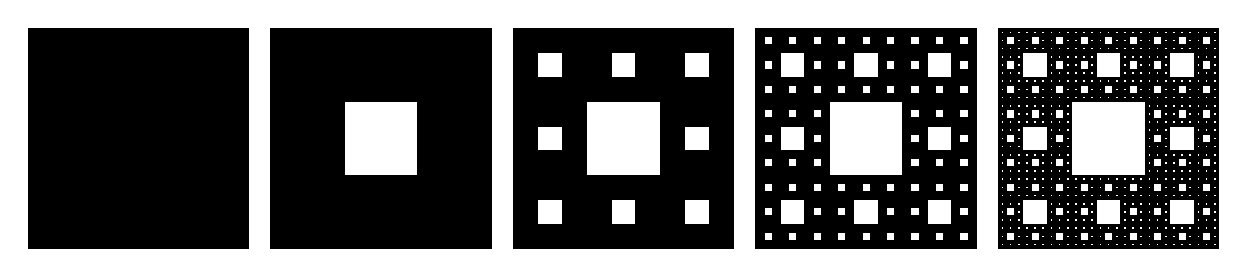
\begin{tikzpicture}[scale=2.8]
    \foreach\i in {0,...,\if\longSierp14\else1\fi} {
    \begin{scope}[shift={(\i*1.1,0)}]
      \sierp{\i}
    \end{scope}}
  \end{tikzpicture}

  
  Napíš program, ktorý zo vstupu prečíta $n$ a vyrobí obrázok rozmerov
  $3^n\times3^n$ (t.j. úroveň 0 má stranu dĺžky $1$, úroveň $1$ stranu $3$,
  a úroveň $n$ stranu $3^n=\overbrace{3\cdot3\cdots3}^n$), v ktorom bude koberec úrovne $n$.
\end{uloha}

